\section{Decision Trees} 

  In here, we define the decision tree model. It is most natural for classification, but there are variants of it for regression.   

  Many discriminative models can be written in a clean formula (e.g. $y = w^T x + \epsilon$ for linear regression, and even $y = \prod_i (\sigma_i \circ A_i) (x)$ for MLPs). However, we cannot find such a parameteric form for a tree, which is why they are nonparametric models. In full generality, all we can say is that they have a general tree structure, and there are many variants. 

\subsection{Classification Trees}

  \begin{definition}[Classification Trees] 
    A \textbf{decision/classification tree} is a nonparameteric discriminative model $f$ that creates some sort of tree representing a set of decisions on an input $x$ to predict a label $y$. 

    \begin{figure}[H]
      \centering 
      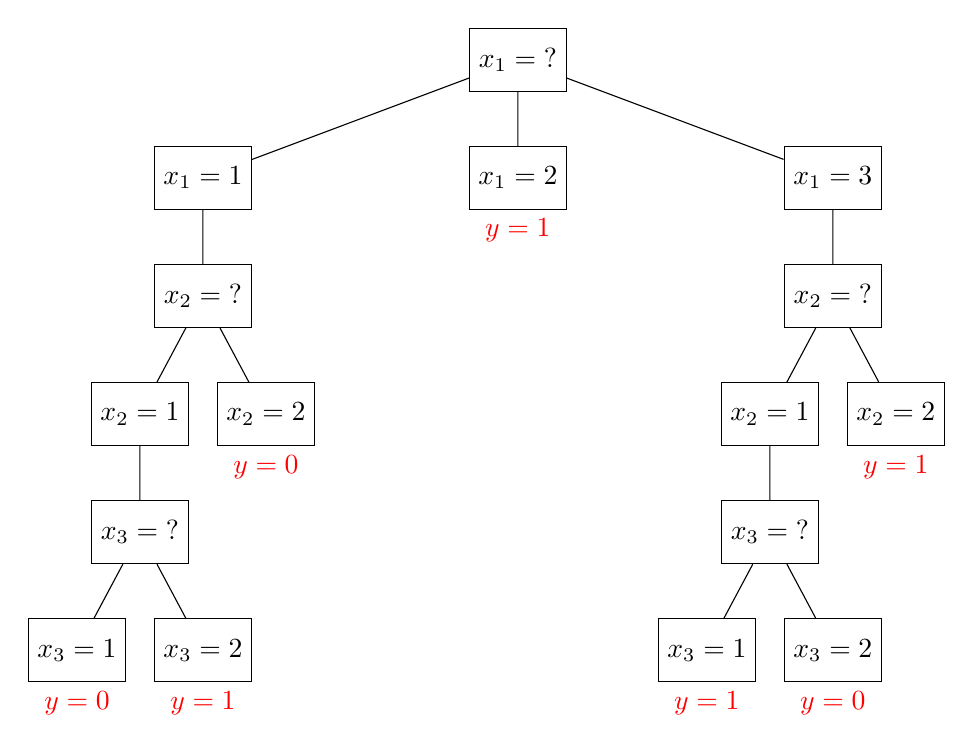
\begin{tikzpicture}[
        level 1/.style={sibling distance=40mm},  % Increased from 48mm
        level 2/.style={sibling distance=20mm},  % Increased from 16mm
        level 3/.style={sibling distance=16mm},  % Increased from 8mm
        box/.style={draw, rectangle, minimum width=12mm, minimum height=8mm},
        edge from parent/.style={draw, -}  % Added for cleaner look
      ]
        \node[box] {$x_1=\text{ ?}$}
          % Level 1
          child {
            node[box] {$x_1=1$}
            child {
              node[box] {$x_2=\text{ ?}$}
              child {
                node[box] {$x_2=1$}
                child {
                  node[box] {$x_3=\text{ ?}$}
                  child {
                    node[box] {$x_3=1$}
                    node[below=4mm] {\textcolor{red}{$y=0$}}
                  }
                  child {
                    node[box] {$x_3=2$}
                    node[below=4mm] {\textcolor{red}{$y=1$}}
                  }
                }
              }
              child {
                node[box] {$x_2=2$}
                node[below=4mm] {\textcolor{red}{$y=0$}}
              }
            }
          }
          % Middle branch
          child {
            node[box] {$x_1=2$}
            node[below=4mm] {\textcolor{red}{$y=1$}}
          }
          % Right branch
          child {
            node[box] {$x_1=3$}
            child {
              node[box] {$x_2=\text{ ?}$}
              child {
                node[box] {$x_2=1$}
                child {
                  node[box] {$x_3=\text{ ?}$}
                  child {
                    node[box] {$x_3=1$}
                    node[below=4mm] {\textcolor{red}{$y=1$}}
                  }
                  child {
                    node[box] {$x_3=2$}
                    node[below=4mm] {\textcolor{red}{$y=0$}}
                  }
                }
              }
              child {
                node[box] {$x_2=2$}
                node[below=4mm] {\textcolor{red}{$y=1$}}
              }
            }
          };
      \end{tikzpicture}
      \caption{An example of a decision tree that splits at $x_1$ first, then $x_2$, and finally $x_3$. Note that you can still split on $x_2$ if $x_1 = 1$ and $x_3$ if $x_1 = 3$. } 
      \label{fig:decision_tree}
    \end{figure}
  \end{definition}

  The decision tree tries to take advantage of some nontrivial covariance between $X$ and $Y$ by constructing nested partitions of the dataset $\mathcal{D}$, and within a partition, it predicts the label that comprises the majority. 

  \begin{example}[Restaurant Dataset]
    Consider the following dataset, where we consider a binary classification system with discrete covariates. 

    \begin{table}[H]
      \centering
      {\footnotesize 
      \begin{tabular}{|c|c|c|c|c|c|c|c|c|c|c|}
        \hline
        & OthOptions & Weekend & WaitArea & Plans & Price & Precip & Restaur & Wait & Crowded & Stay? \\
        \hline
        $x_1$ & \textcolor{blue}{Yes} & \textcolor{blue}{No} & \textcolor{blue}{No} & \textcolor{blue}{Yes} & \$\$\$ & \textcolor{blue}{No} & \textcolor{blue}{Mateo} & 0-5 & \textcolor{blue}{some} & Yes \\
        \hline
        $x_2$ & \textcolor{green!50!black}{Yes} & \textcolor{green!50!black}{No} & \textcolor{green!50!black}{No} & \textcolor{green!50!black}{Yes} & \$ & \textcolor{green!50!black}{No} & \textcolor{green!50!black}{Juju} & 16-30 & \textcolor{green!50!black}{full} & No \\
        \hline
        $x_3$ & \textcolor{blue}{No} & \textcolor{blue}{No} & \textcolor{blue}{Yes} & \textcolor{blue}{No} & \$ & \textcolor{blue}{No} & \textcolor{blue}{Pizza} & 0-5 & \textcolor{blue}{some} & Yes \\
        \hline
        $x_4$ & \textcolor{blue}{Yes} & \textcolor{blue}{Yes} & \textcolor{blue}{No} & \textcolor{blue}{Yes} & \$ & \textcolor{blue}{No} & \textcolor{blue}{Juju} & 6-15 & \textcolor{blue}{full} & Yes \\
        \hline
        $x_5$ & \textcolor{green!50!black}{Yes} & \textcolor{green!50!black}{Yes} & \textcolor{green!50!black}{No} & \textcolor{green!50!black}{No} & \$\$\$ & \textcolor{green!50!black}{No} & \textcolor{green!50!black}{Mateo} & 30+ & \textcolor{green!50!black}{full} & No \\
        \hline
        $x_6$ & \textcolor{blue}{No} & \textcolor{blue}{No} & \textcolor{blue}{Yes} & \textcolor{blue}{Yes} & \$\$ & \textcolor{blue}{Yes} & \textcolor{blue}{BlueCorn} & 0-5 & \textcolor{blue}{some} & Yes \\
        \hline
        $x_7$ & \textcolor{green!50!black}{No} & \textcolor{green!50!black}{No} & \textcolor{green!50!black}{Yes} & \textcolor{green!50!black}{No} & \$ & \textcolor{green!50!black}{Yes} & \textcolor{green!50!black}{Pizza} & 0-5 & \textcolor{green!50!black}{none} & No \\
        \hline
        $x_8$ & \textcolor{blue}{No} & \textcolor{blue}{No} & \textcolor{blue}{No} & \textcolor{blue}{Yes} & \$\$ & \textcolor{blue}{Yes} & \textcolor{blue}{Juju} & 0-5 & \textcolor{blue}{some} & Yes \\
        \hline
        $x_9$ & \textcolor{green!50!black}{No} & \textcolor{green!50!black}{Yes} & \textcolor{green!50!black}{Yes} & \textcolor{green!50!black}{No} & \$ & \textcolor{green!50!black}{Yes} & \textcolor{green!50!black}{Pizza} & 30+ & \textcolor{green!50!black}{full} & No \\
        \hline
        $x_{10}$ & \textcolor{green!50!black}{Yes} & \textcolor{green!50!black}{Yes} & \textcolor{green!50!black}{Yes} & \textcolor{green!50!black}{Yes} & \$\$\$ & \textcolor{green!50!black}{No} & \textcolor{green!50!black}{BlueCorn} & 6-15 & \textcolor{green!50!black}{full} & No \\
        \hline
        $x_{11}$ & \textcolor{green!50!black}{No} & \textcolor{green!50!black}{No} & \textcolor{green!50!black}{No} & \textcolor{green!50!black}{No} & \$ & \textcolor{green!50!black}{No} & \textcolor{green!50!black}{Juju} & 0-5 & \textcolor{green!50!black}{none} & No \\
        \hline
        $x_{12}$ & \textcolor{blue}{Yes} & \textcolor{blue}{Yes} & \textcolor{blue}{Yes} & \textcolor{blue}{Yes} & \$ & \textcolor{blue}{No} & \textcolor{blue}{Pizza} & 16-30 & \textcolor{blue}{full} & Yes \\
        \hline
      \end{tabular}
      }
      \caption{Dataset of whether to go to a restaurant for a date depending on certain factors. }
      \label{tab:restaurant}
    \end{table}

    Let us denote $\mathcal{D}$ as the dataset, and say that $F_1, \ldots, F_d$ were the features. This is a binary classification problem, and we can count that there are $6$ positives and $6$ negative labels. 
  \end{example}

  Note that this model is extremely flexible in that we can have different properties of these trees. We will introduce them as we go. 

  \begin{definition}[Binary Decision Tree]
    A \textbf{binary decision tree} only allows the tree to split into two nodes. 
  \end{definition} 

  Note that in density estimation or linear regression, we can derive the risk by first deriving the likelihood of the data, and then taking the negative logarithm of it to get our loss function which allows us to define our risk. In a decision tree, we have a \textit{non-probabilistic} discriminative model, so there is no concept of likelihood. Therefore, we cannot use a pdf to define the loss. Fortunately, we can use the straightforward misclassification risk. 

  \begin{theorem}[Expected and Empirical Risk of Decision Trees]
    Given a classification tree $f$, the misclassification risk over the true data generating distribution $p(x, y)$, along with its empirical risk over a dataset $\mathcal{D} = (x^{(i)}, y^{(i)})_{i=1}^n$, is 
    \begin{align}
      \mathbb{R}(f) & = \mathbb{E}_{x, y} \left[ \mathbbm{1} (y \neq f(x))\right] = \int \mathbbm{1} (y \neq f(x)) \, dx \,dy \\ 
      \hat{R}(f) & = \frac{1}{n} \sum_{i=1}^n \mathbbm{1} (y^{(i)} \neq f(x^{(i)}))
    \end{align}
    where $\mathbbm{1}(p)$ is an indicator function that equals $1$ if $p$ is true and $0$ if false. Note that $\hat{R}(f)$ is simply 1 minus the accuracy. 
  \end{theorem} 

  This is all nice in theory, but how are we supposed to optimize this in practice? First, the misclassification loss is not differentiable---and even worse---the gradient is $0$ almost everywhere! This can be solved by using a surrogate loss function. Even worse, $f$ is not parameteric, so we can't even gradients at all (with respect to what parameter?)! Another solution is to try and create a very specific tree model---making it parameteric---and then using a surrogate loss to learn. In fact this is what some people do, but for now we keep things simple. Therefore, we must use a gradient-free rule to optimize a decision tree. 

\subsection{Regression Trees}

\subsection{Model Space} 

  The fact that trees are nonparameteric means that we have extreme flexibility in designing our tree. However, this comes with the big risk of having too big of a model space to optimize over. This overcomplexity is one of the big challenges in trees. 

  For example, suppose that there are $d$ covariates (independent variables, features) $x_1, \ldots, x_d$ all binary valued. We can design a decision tree that splits on $x_1$, then on $x_2$, then on $x_1$, then on $x_2$, and so on. This becomes unbounded and our model space a discrete infinite space, which is a bad combination since we don't have gradients to optimize over a continuum. We can try and handle this in two ways. 

  \begin{example}[Splitting on Same Variable Multiple Times]
    Splitting on covariate $x_1$ infinitely many times seems pretty unrealistic, so we should limit it in some way. 
    \begin{enumerate}
      \item \textit{Covariate can be split a maximum of once for each path from root to leaf}. This is a 
      \item \textit{Covariate can be split maximum of $k$ times}. 
    \end{enumerate}
  \end{example}

  \begin{example}[Depth of Tree]
    
  \end{example} 

  \begin{example}[Max Subnodes per Split]
    
  \end{example}
